%% LyX 2.4.0~beta5 created this file.  For more info, see https://www.lyx.org/.
%% Do not edit unless you really know what you are doing.
\documentclass[english,footrule]{foils}
\usepackage[T1]{fontenc}
\usepackage[latin9]{inputenc}
\pagestyle{foilheadings}
\setcounter{secnumdepth}{1}
\setcounter{tocdepth}{1}
\usepackage{color}
\usepackage{cprotect}
\usepackage{pifont}
\usepackage{url}
\usepackage{amsmath}
\usepackage{amsthm}
\usepackage{amssymb}
\usepackage{graphicx}

\makeatletter
%%%%%%%%%%%%%%%%%%%%%%%%%%%%%% Textclass specific LaTeX commands.
\theoremstyle{definition}
\newtheorem{defn}{\protect\definitionname}
\theoremstyle{plain}
\newtheorem{fact}{\protect\factname}
\theoremstyle{remark}
\newtheorem{rem}{\protect\remarkname}

%%%%%%%%%%%%%%%%%%%%%%%%%%%%%% User specified LaTeX commands.
\newcommand{\argmin}{\operatornamewithlimits{argmin}}

\usepackage{xcolor}
\renewcommand{\labelitemi}{$\textcolor{blue}{\bullet}$}
\renewcommand{\labelitemii}{$\textcolor{teal}{\Rightarrow}$}
\renewcommand{\labelitemiii}{$\textcolor{red}{\rightarrow}$}
\renewcommand{\labelitemiv}{$\textcolor{brown}{\circ}$}

\newcommand{\T}{\mathrm{T}}  % transpose
\newcommand{\PP}{\mathrm{P}}  % probability
\newcommand{\dd}{\mathrm{d}} % integration dx
\newcommand{\ee}{\mathrm{e}} % exponential
\newcommand{\E}{\mathrm{E}} % expectation

\makeatother

\usepackage{babel}
\providecommand{\definitionname}{Definition}
\providecommand{\factname}{Fact}
\providecommand{\remarkname}{Remark}

\begin{document}

\MyLogo{Intro ML--Resampling and Tuning}
\title{Resampling and Tuning\\
\rule[0.5ex]{1\columnwidth}{3pt}}
\author{Mark Asch - IMU/VLP/CSU }
\date{2023}
\maketitle

\foilhead{Resampling Methods: Motivation}
\begin{itemize}
\item Resampling is an \textcolor{magenta}{indispensable} tool of machine
learning and modern statistics. 
\item It provides an evaluation of two important aspects of a general statistical
model:
\begin{enumerate}
\item The \textcolor{magenta}{predictive performance} of a given model. 
\item \textcolor{magenta}{Tuning} of the \textcolor{magenta}{method parameters}
to find an optimal set. 
\end{enumerate}
\item It is the best way to avoid \textcolor{magenta}{data leakage}, or
data ``crimes,'' where the same data that was used to construct,
or train the model, is used to test, or evaluate it. 
\begin{itemize}
\item In other words, it is considered\textcolor{red}{{} bad practice} to
provide accuracy or predictive performance measures of a statistical
method based on the data that was used to estimate the model. 
\item We should always attempt an objective evaluation of our models. 
\item Note that data leakage can also occur during stages of data preparation. 
\item An example is the use of all the data to perform normalization. One
should normalize at the level of the training samples, since otherwise
there is information leaking into the model from outside its scope. 
\item The result will be an overly-optimistic, or\textcolor{magenta}{{} overfitted
}model. 
\item A model obtained in this way will often be useless in reality.
\end{itemize}
\end{itemize}

\foilhead{Resampling Methods: Procedure}
\begin{itemize}
\item The basic procedure of any resampling method is:
\begin{enumerate}
\item Draw \textcolor{magenta}{samples}, repeatedly, from a \textcolor{magenta}{training}
set. 
\item \textcolor{magenta}{Refit }a model on each sample. 
\item Compute an average, or \textcolor{magenta}{best model}. 
\item Apply this model to\textcolor{magenta}{{} test sets}, which are complementary
subsets that have \textcolor{magenta}{not }been used in the training
phase. 
\end{enumerate}
\end{itemize}

\foilhead{Resampling Methods: Cross-Validation}
\begin{itemize}
\item The most commonly-used resampling technique is \textcolor{magenta}{cross-validation}
(CV), depicted in the Figure below. 
\item It is used for:
\begin{itemize}
\item \textcolor{magenta}{Model evaluation}, when the test error associated
with a ML method is used to measure its performance. 
\item \textcolor{magenta}{Model selection/tuning}, when a suitable level
of flexibility of the model is to be chosen by varying its \textcolor{magenta}{hyperparameters}. 
\end{itemize}
\item CV has the following forms:
\begin{itemize}
\item $k$-fold, 
\item train/test split ($k=2$ ), 
\item LOOCV ($k=n$ ), 
\item stratified CV, 
\item repeated CV. 
\end{itemize}
%
\end{itemize}
\begin{figure}
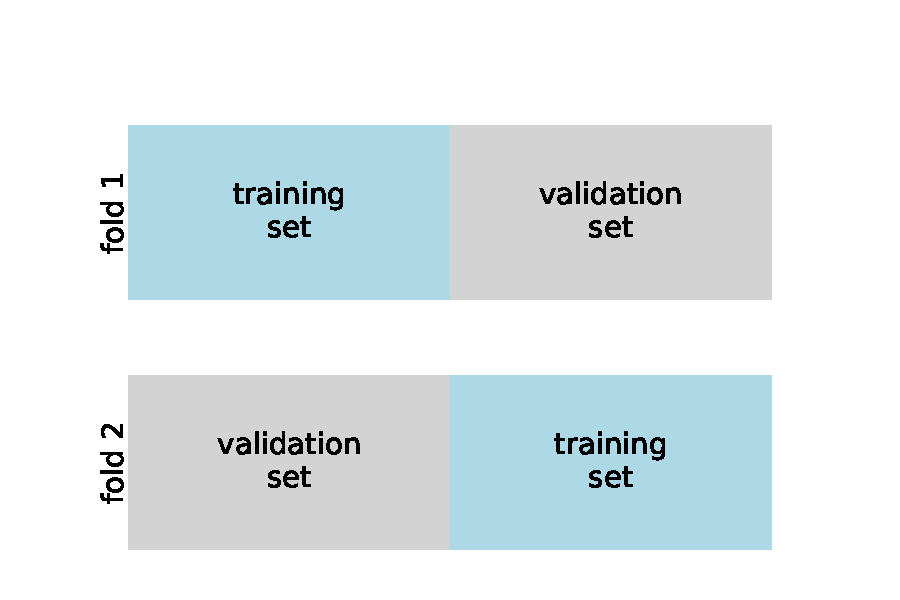
\includegraphics[width=0.5\textwidth]{graphics/k-2-fold-CV}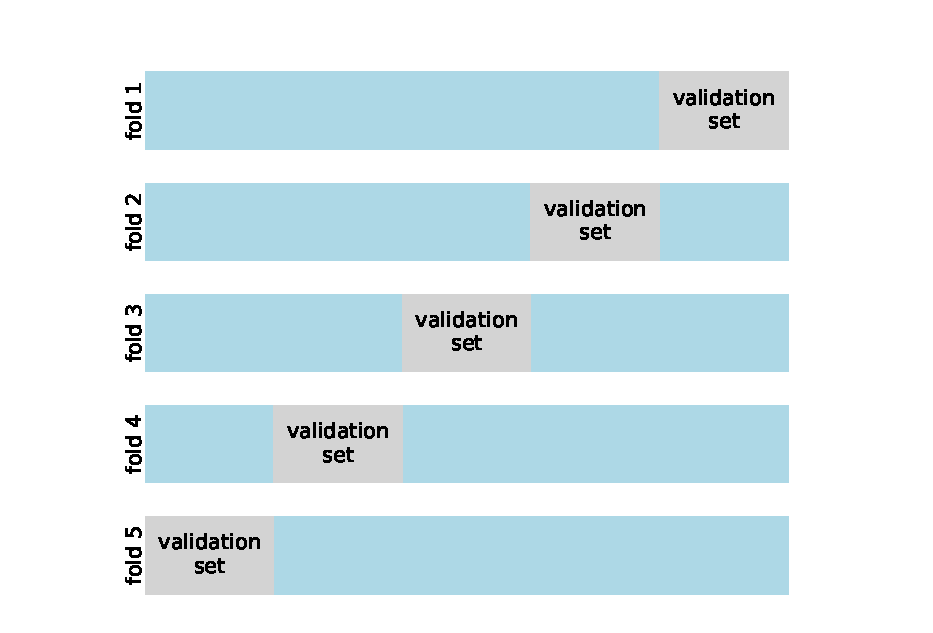
\includegraphics[width=0.5\textwidth]{graphics/k-5-fold-CV}

\caption{{2-fold (left) and 5-fold CV (right). Training set is blue, validation
set is gray.}}
\end{figure}


\foilhead{Resampling Methods: Bootstrap}
\begin{itemize}
\item A second resampling approach is called \textcolor{magenta}{bootstrap}. 
\item This is used when we want to provide a measure of accuracy, or \textcolor{magenta}{quantify
the uncertainty} of any statistical learning method.
\item Bootstrap is based on sampling with \textcolor{magenta}{replacement}---see
below.
\end{itemize}

\foilhead{$\;$}

\vfill{}

\begin{center}
{\Large\textbf{\textcolor{blue}{1. CROSS-VALIDATION}}}{\Large\par}
\par\end{center}

\vfill{}


\foilhead{Cross-Validation }
\begin{defn}
[Cross-Validation] CV is a class of methods for estimating the \textcolor{magenta}{test
error} rate of a statistical model by retaining a subset of the training
observations from the fitting process, then applying the computed
model to these retained observations.
\end{defn}
\begin{center}
\includegraphics[scale=0.25]{\string"/Users/markasch/Documents/Refs/Statistics and Data Science/Kuhn-Johnson/APM/APM_Figures-master/Chapter_04_Over-Fitting_and_Model_Tuning/Ch04Fig06\string".png}
\par\end{center}
\begin{itemize}
\item The accepted practice for all ML methods is to learn the model on
a \textcolor{magenta}{training set} of observations, then test the
learned model on an unseen \textcolor{magenta}{test set }of new observations,
thus directly estimating the test error rate. 
\item But often we only have the training set available. To compensate for
this, there are a number of \textcolor{magenta}{cross-validation}
techniques that can be employed to estimate the test error rate using
the available training data-
\item Cross-validation should be used \textcolor{magenta}{systematically}.
\end{itemize}

\foilhead{1. Cross-Validation: properties}

CV has the following properties: 
\begin{itemize}
\item \textcolor{magenta}{simple} to understand 
\item relatively \textcolor{magenta}{straightforward} to implement---most
ML libraries and routines have built-in CV methods. 
\item provides an estimation with less bias and potentially less variance,
though there is a \textcolor{magenta}{trade-off}---see below. 
\item provides a\textcolor{magenta}{{} less ``optimistic''} estimation than
a simple, single train-test partition of the observation data. 
\end{itemize}
\begin{fact}
CV is an essential tool in all statistical learning methods for evaluating
the confidence in the model and producing as robust a model as possible
that will perform well on future, unseen data. 
\end{fact}

\foilhead{1. Cross-Validation: variants}
\begin{flushleft}
\textcolor{magenta}{A. Validation Set CV.}
\par\end{flushleft}

\index{machine learning!cross-validation!validation set} This is
the simplest form of CV. 
\begin{itemize}
\item Randomly divide the set of observations into two parts: a training
set and a validation set. 
\item Fit the model using the training set, and use the fitted model to
predict the responses for the observations in the validation set. 
\item The resulting error rate of the validation---typically estimated
by the MSE---provides an estimation of the test error rate. 
\end{itemize}
\textcolor{magenta}{B. Leave-One-Out Cross-Validation (LOOCV)}

\index{machine learning!cross-validation!LOOCV} 
\begin{itemize}
\item A single observation $(x_{1},y_{1})$ is used for the validation set. 
\item The remaining observations,${(x_{2},y_{2}),...,(x_{n},y_{n})},$ constitute
the training set. 
\item Then cycle through the indices, $i=2,\ldots,n.$ 
\end{itemize}
\textcolor{magenta}{C. $k$-Fold Cross-Validation}

\index{machine learning!cross-validation!kf@$k$-fold} 
\begin{itemize}
\item Randomly divide the set of observations into $k$ groups, called \emph{folds},
of the same size. 
\item The first group becomes the validation set. 
\item The method is fit on the $k-1$ remaining groups. 
\item The validation set approach is the special case, $k=2.$ LOOCV is
the special case, $k=n.$ 
\end{itemize}
One usually performs $k$-fold cross validation with $k=5$ or $k=10,$
as described in the Algorithm below.
\begin{center}
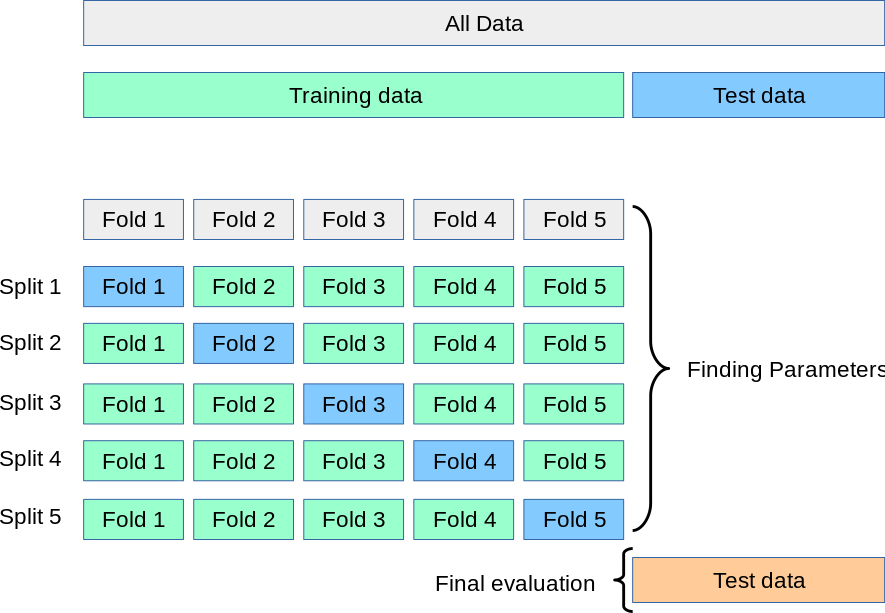
\includegraphics[width=1\textwidth]{graphics/k-fold}
\par\end{center}


\foilhead[-0.5in]{CV Algorithm: Train/Test (Validation) Splits}
\begin{enumerate}
\item Divide the data into two subsets: 
\begin{enumerate}
\item a training set (usually 80\%), 
\item a validation set (usually 20\%) that plays the role of a test set. 
\end{enumerate}
\item Fit the model to the training subset. 
\item Compute the mean-square error of the model applied to the validation
subset. 
\item Compare with the MSE of the training subset. 
\item Modify the sample size, and repeat. 
\end{enumerate}

\foilhead[-0.5in]{CV Algorithm: k-fold}
\begin{enumerate}
\item Divide the full data set randomly into $k$ groups, called folds. 
\item Fit the data on all the folds, except the first one. 
\item Compute the mean squared error on the ``left out'' fold (the validation
set). 
\item Repeat the above two steps and compute $k$ estimates of the test
error, $\mathrm{MSE}_{1},\mathrm{MSE}_{2},\ldots,\mathrm{MSE}_{k}.$ 
\item Finally, compute the $k$-fold cross-validation error estimate as
the average, 
\[
\mathrm{CV}_{(k)}=\frac{1}{k}\sum_{i=1}^{k}\mathrm{MSE}_{i}.
\]
\end{enumerate}

\foilhead{Mesures of Performance}
\begin{itemize}
\item To begin with, we require individual performance scores for each cycle
of the CV loop.
\begin{itemize}
\item For regression problems, use the \textcolor{magenta}{mean squared
error}\index{machine learning!cross-validation!mean squared error (MSE)}
\[
\mathrm{MSE}=\frac{1}{n}\sum_{i=1}^{n}\left(y_{i}-\hat{y}_{i}\right)^{2},
\]
where $\hat{y}_{i}$ is the predicted value by the model for observation
$i.$ 
\item For classification problems, use the \textcolor{magenta}{misclassification
rate}\index{machine learning!cross-validation!misclassification rate (MCE)}
\[
\mathrm{MCE}=\frac{1}{n}\sum_{i=1}^{n}I\left(y_{i}\ne\hat{y}_{i}\right),
\]
where $\hat{y}_{i}$ is the class, or label predicted by the model
for observation $i.$ 
\end{itemize}
\item Then, the \textcolor{magenta}{general score} of the CV is the average
of the $k$ individual scores, 
\[
\mathrm{CV}_{(k)}=\frac{1}{k}\sum_{j=1}^{k}\mathrm{MSE}_{j},
\]
to which we add a measure of the variance, the \textcolor{magenta}{standard
error,} which is the standard deviation of the sampling distribution,
\[
\mathrm{SE}=\frac{s}{\sqrt{n}},
\]
where $s$ is the empirical standard deviation, the square root of
the empirical variance, 
\[
s^{2}=\frac{1}{n-1}\sum_{i=1}^{n}\left(x_{i}-\bar{x}\right)^{2}.
\]
\item Finally, an estimated 95\% \textcolor{magenta}{confidence interval
}of the empirical mean\footnote{This confidence interval is exact for a Gaussian distribution, but
random i.i.d. errors and their sums are only approximately Gaussian.}, is defined by 
\[
\bar{x}\pm1.96\mathrm{SE}.
\]
\end{itemize}

\foilhead{Cross-Validation - remarks on $k$-Fold Cross-Validation}
\begin{itemize}
\item \textcolor{magenta}{\emph{Bias-Variance Compromise}}: $k$-fold CV
provides more accurate estimates of the test error rate than LOOCV,
thanks to the trade-off that causes a smaller bias for LOOCV, but
larger variance. 
\item Any \textcolor{magenta}{\emph{normalization}}, prior to fitting the
model, should be performed within the loop and not over all the data,
otherwise there is a risk of producing overly optimistic estimations---see
the discussion on data leakage below. 
\item Each observation is affected to a \textcolor{magenta}{unique }group
or fold, and remains in its group for the remainder of the procedure. 
\end{itemize}

\foilhead{Cross-Validation - Choice of $k$}
\begin{itemize}
\item The value of $k$ must be \textcolor{magenta}{chosen with care}, depending
on the context. 
\item Desired properties are: 
\begin{itemize}
\item The value must be \textcolor{magenta}{\emph{representative}}, meaning
that $k$ should be chosen so that each train/test group is sufficiently
large to contain a representative sample of all the data. 
\item \textcolor{magenta}{$k=10$} is the value, found by experience, that
produces a performance estimation with small bias and modest variance. 
\item \textcolor{magenta}{$k=5$} is often used to compensate for smaller
values of $n.$ 
\end{itemize}
\end{itemize}

\foilhead{Cross-Validation - Variants of CV}

\index{machine learning!cross-validation!variants} 
\begin{description}
\item [{\emph{Train/test}}] \emph{split}: one extreme, where $k=2.$ 
\item [{\emph{LOOCV}:}] the other extreme, where $k=n,$ usable only when
$n$ is not too large. 
\item [{\emph{Stratified}:}] the split ensures that each fold contains
the same proportion of observations of each class. 
\item [{\emph{Repeated}:}] repeat the $k$-fold cross-validation $M$ times,
usually 3, 5, or 10, where the data are randomly reshuffled prior
to each repetition, thus resulting in different splits each time. 
\item [{\emph{Repeated}}] \emph{Train/test}: divide into train/test, then
repeat the division multiple times---this requires a greater number
of repetitions than the $k$-fold method. 
\end{description}
\begin{dinglist}{52}
\item Recommended when datasets are small and models are simple.
\item Produces a more stable estimation of the average performance.
\end{dinglist}
\begin{description}
\item [{\emph{Nested}:}] perform a CV with $k$-folds within each fold---often
used for tuning hyperparameters during model validation. 
\end{description}

\foilhead{Cross-Validation -Train-Test Split or $k$-Fold?}
\begin{itemize}
\item Train-Test is the simplest version of $k$-fold CV, with $k=2.$ It
is used mainly when $n$ is large and the training cost is high, e.g.,
in deep neural networks. It is not suited to small values of $n$
for which one should always use classical $k$-fold. The split {proportion}
is chosen as a function of
\begin{itemize}
\item computational cost of the training, 
\item computational cost of model evaluation. 
\item representativity of the training set, 
\item representativity of the test set. 
\end{itemize}
\item The usual values are:
\begin{itemize}
\item train 80\%, test 20\%, 
\item train 67\%, test 33\%, 
\item train 50\%, test 50\%. 
\end{itemize}
\end{itemize}

\foilhead{Implementations of CV}

There are a few possibilities. 
\begin{itemize}
\item Code it by hand, either with Python or R---see Example below. 
\item Use the \texttt{caret}\footnote{\url{https://CRAN.R-project.org/package=caret}}
package of R---see below for a brief presentation of this extremely
useful package. 
\item Use the \texttt{cross\_validate}\cprotect\footnote{\url{https://scikit-learn.org/stable/modules/cross_validation.html}}
function of \texttt{scikit-learn}. 
\end{itemize}

\foilhead{$\;$}

\vfill{}

\begin{center}
{\Large\textbf{\textcolor{blue}{2. BOOTSTRAPPING}}}{\Large\par}
\par\end{center}

\vfill{}


\foilhead{2. Bootstrap}
\begin{defn}
A bootstrap method is a resampling technique used to estimate population
statistics by repeatedly resampling a dataset with \emph{replacement}.
\end{defn}
\begin{itemize}
\item Bootstrapping has classically been used to estimate summary statistics
of a sample, such as means or standard deviations. 
\item In ML it can be used to estimate the predictive performance on unseen
data, as an alternative to CV. 
\item The chief advantage of bootstrap is that it provides \textcolor{magenta}{\emph{confidence
intervals}} for the estimates that are not available from a simple
CV.
\end{itemize}
\begin{fact}
Sampling with replacement has the remarkable property that the samples
drawn will include approximately $62$\% of the observations only,
thus leaving an \textcolor{magenta}{\emph{out-of-bag}} sample, consisting
of the approximately $38$\% of unused observations, that can then
be used as a test set.
\end{fact}

\foilhead{Bootstrap - confidence intervals}
\begin{itemize}
\item Bootstrap provides an idea of the\textcolor{magenta}{{} confidence interval}
of an estimation. 
\item A bootstrap confidence interval, of\textcolor{magenta}{\emph{ level
${\displaystyle \alpha},$}} is computed by identifying the percentiles
of the bootstrap distribution, leaving on both sides of the distribution
${\displaystyle \alpha/2\times100\%.}$ 
\begin{itemize}
\item to obtain a good bootstrap confidence interval, the \textcolor{magenta}{\emph{number
of simulations}} must be big enough, usually of the order of ${\displaystyle N\geq1000}$ 
\end{itemize}
\item Bootstrap is applicable to a large variety of supervised learning
methods, especially when a method does not provide \textcolor{magenta}{\emph{measures
of variability}}
\end{itemize}

\foilhead{Bootstrap - algorithm}
\begin{enumerate}
\item Choose the number $N$ of bootstrap samples to perform. 
\item Choose a sample size $n_{b}$ from the $n$ available observations,
with $n_{b}\le n.$ 
\item For each bootstrap sample: 
\begin{enumerate}
\item Draw a sample with replacement with the chosen size $n_{b}.$ 
\item Fit a model on the data sample. 
\item Estimate the predictive skill of the model on the \textcolor{magenta}{\emph{out-of-bag
}}sample. 
\end{enumerate}
\item Calculate the mean of the sample of model skill estimates. 
\item Calculate a \textcolor{magenta}{\emph{confidence interval }}on the
mean. 
\end{enumerate}
\begin{itemize}
\item The confidence interval can be computed parametrically, or non-parametrically. 
\begin{itemize}
\item In the former, we suppose an approximate Gaussian sampling distribution
and use the standard $\mathcal{N}(0,1)$ confidence limits. 
\item The non-parametric approach simply requires the ordering of the values,
followed by the identification of the chosen quantiles according to
the confidence level chosen. 
\end{itemize}
\end{itemize}

\foilhead{Bootstrap - remarks}

Some important remarks are: 
\begin{itemize}
\item The bootstrap is applicable to most statistical learning methods,
especially when there are no measures of uncertainty available. 
\item Due to the sampling with replacement, a bootstrapped dataset may contain
multiple instances of the same original observations, and may completely
omit other original observations. 
\item To obtain a reliable confidence interval, a large number of simulations
must be performed, usually $N>1000.$ This will not be feasible for
computationally expensive models. 
\item Though one usually takes the bootstrap sample size $n_{b}$ equal
to the totality of the available samples, $n,$ this can be reduced
to $50$\% or $80$\% of the original dataset in the case where $n$
is very large. 
\end{itemize}

\foilhead{Implementations of Bootstrap}

The function calls are: 
\begin{description}
\item [{\textcolor{blue}{R}}]~
\end{description}
\begin{verbatim}
	library(boot)
	bootobject <- boot(data= , statistic= , R=N, ...) 	
	
\end{verbatim}
\begin{description}
\item [{\textcolor{blue}{scikit}}]~
\end{description}
\begin{verbatim}
	from sklearn.utils import resample
	boot = resample(data, replace=True, 
         n_samples=N, random_state=1)
     
\end{verbatim}

\foilhead{Cross Validation vs. Bootstrapping}
\begin{itemize}
\item Both cross validation and bootstrapping are resampling methods.
\begin{itemize}
\item Cross-Validation provides estimates of the test error. 
\item Bootstrap provides, in addition, the standard error of the estimates. 
\end{itemize}
\item As the name cross-validation suggests, its primary purpose is measuring
(generalization) performance of a model. 
\item By contrast, bootstrapping is primarily used to establish empirical
distribution functions for a widespread range of statistics, ranging
from the variation of the mean to the variation of models in bagged
ensemble models. 
\item The bootstrap equivalent to cross-validation estimates of the predictive
performance error is called an out-of-bootstrap, or out-of-bag (OOB)
estimate.
\end{itemize}
\begin{rem}
In practice there is often not much of a difference between iterated
$k$-fold cross-validation and out-of-bootstrap. With a similar total
number of evaluated sampling models, the model prediction error measurement
is similar, although OOB typically has more bias and less variance
than the corresponding CV estimates.
\end{rem}

\foilhead{Resampling: Take-Home Lessons}

No resampling method is uniformly better than another and the choice
of a particular method should consider several aspects.
\begin{itemize}
\item If the \textcolor{magenta}{sample size is small}, repeated 10-fold
cross-validation is recommended for several reasons: the bias and
variance properties are good and, given the sample size, the computational
costs are not large. 
\item If the goal is to \textcolor{magenta}{choose between models}, as opposed
to getting the best indicator of performance, it is advisable to use
a bootstrap method since these have very low variance. 
\item For \textcolor{magenta}{large sample sizes}, the differences between
resampling methods become less pronounced, and computational efficiency
becomes the critical factor. Here, simple 10-fold cross-validation
should provide acceptable variance and low bias, and is relatively
cheap to compute. 
\end{itemize}

\foilhead{The R command \texttt{\textcolor{blue}{boot}} }
\begin{itemize}
\item the pacakge \texttt{\textcolor{blue}{boot}} provides numerous possibilities
for obtaining bootstrap estimations 
\item command and arguments:
\begin{itemize}
\item \texttt{\textcolor{blue}{bootobject <- boot(data = , statistic = ,
R = , ...)}}
\begin{itemize}
\item \texttt{\textcolor{blue}{data}} is a vector, matrix or dataframe
\item \texttt{\textcolor{blue}{statistic}} is a function that gives the
$k$ statistics to be bootdtrapped; the function must include a parameter/argument
\texttt{\textcolor{blue}{indices }}so that \texttt{\textcolor{blue}{boot}}
can choose the cases for each replica
\end{itemize}
\item \texttt{\textcolor{blue}{R}} the number of repeats of the - normaly
around $1000$ (at least)
\end{itemize}
\item \texttt{\textcolor{blue}{boot()}} calls the function <<statistic>>
R times, each time using sampling with replacement, and the statistics
are computed and stored in the structure \texttt{\textcolor{blue}{bootobject}}
that contains
\begin{itemize}
\item \texttt{\textcolor{blue}{t0}} are the observed values of the $k$
statistics applied to the original data
\item \texttt{\textcolor{blue}{t}} is a matrix $R\times k,$ where each
row is a bootstrap replicaof the $k$ statistics
\end{itemize}
\item outputs:
\begin{itemize}
\item \texttt{\textcolor{blue}{print(bootobjet)}}
\item \texttt{\textcolor{blue}{plot(bootobjet)}}
\end{itemize}
\item confidence intervals: if the outputs are acceptable, then the confidence
intervals can be calculated by
\begin{itemize}
\item \texttt{\textcolor{blue}{boot.ci(bootobjet, conf = , type = )}}
\begin{itemize}
\item \texttt{\textcolor{blue}{conf}} is the level (by default $0.95$)
\item \textcolor{blue}{type} is the distribution: 'norm', 'basic', 'stud',
'perc', 'bca' and 'all' (by default 'all')
\end{itemize}
\end{itemize}
\end{itemize}

\foilhead{$\;$}

\vfill{}

\begin{center}
{\Large\textbf{\textcolor{blue}{3. MODEL TUNING}}}{\Large\par}
\par\end{center}

\vfill{}


\foilhead{3. Model Tuning }
\begin{itemize}
\item Most ML methods require the choice of \textcolor{magenta}{(hyper)parameters}
that cannot be estimated directly from the data.
\item For example,
\begin{itemize}
\item in the \textcolor{magenta}{$k$-nn} classification algorithm, we need
to choose the number of neighbors; 
\item for\textcolor{magenta}{{} SVM} with a radial kernel, we must choose
the exponent; 
\item for \textcolor{magenta}{neural networks}, the complete architecture---layers
and nodes---needs to be chosen, as well as the SGD optimization parameters. 
\end{itemize}
\item These\emph{ tuning parameters} control the \textcolor{magenta}{model
complexity}, and a bad choice will lead to \textcolor{magenta}{overfitting}---see
below. 
\end{itemize}

\foilhead{3. Model Tuning - general approach}
\begin{itemize}
\item To deal with this thorny problem, a general approach that can be applied
to almost any model is:
\begin{itemize}
\item Define a set of \textcolor{magenta}{candidate values }for the parameter(s). 
\item Calculate\textcolor{magenta}{{} robust estimations} of the performance,
usually using \textcolor{magenta}{CV}. 
\item Choose the\textcolor{magenta}{{} optimal parameter} value(s). 
\end{itemize}
\item Then, to obtain \textcolor{magenta}{robust performance estimates}:
\begin{itemize}
\item Divide the date into\textcolor{magenta}{{} training and testing sets
}according to one of the resampling methods and variants seen above. 
\item Choose a candidate set, or \textcolor{magenta}{range of values }for
the parameters---often, tuning methods will provide default ranges,
but these might need to be modified in a given context. 
\item Test the performance over the \textcolor{magenta}{test set.} 
\item Aggregate the results to draw a \textcolor{magenta}{performance profile}. 
\item Select the \textcolor{magenta}{best model}. 
\item Apply the\textcolor{magenta}{{} final model} to all the data, using
the tuning parameters that have just been selected. 
\end{itemize}
\end{itemize}
\begin{center}
\includegraphics[scale=1.25]{\string"/Users/markasch/Documents/Refs/Statistics and Data Science/Kuhn-Johnson/APM/APM_Figures-master/Chapter_04_Over-Fitting_and_Model_Tuning/Ch04Fig04\string".pdf}
\par\end{center}

\foilhead{3. Model Tuning - final parameter choice}
\begin{itemize}
\item Once the model performance has been evaluated over the parameter sets,
there are different approaches for the \textcolor{magenta}{final choice}
of the tuning parameters. 
\begin{itemize}
\item The simplest is to choose the parameters that gave the best performance,
usually based on the average and its standard error.
\item But, to avoid overly complex models, the \textcolor{magenta}{one standard
error }method can be used to choose a simpler model:
\begin{itemize}
\item Identify the optimal model. 
\item Compute its standard error. 
\item Find the \emph{simplest} model within an interval of one standard
error. 
\end{itemize}
\end{itemize}
\item A final approach is to specify a small, acceptable tolerance of the
best value and then choose the simplest model within this tolerance.
\item Example of final choices:
\begin{itemize}
\item simplest approach is to take the best performance estimations
\begin{itemize}
\item here we have 5 repetitions of 10-fold CV, for a total of 50 estimations
of the precision, then we compute the average and its standard error
= $s/\sqrt{n},$ where $s$ is the empirical standard deviation)
\end{itemize}
\end{itemize}
\end{itemize}
\includegraphics{\string"/Users/markasch/Documents/Refs/Statistics and Data Science/Kuhn-Johnson/APM/APM_Figures-master/Chapter_04_Over-Fitting_and_Model_Tuning/Ch04Fig09\string".pdf}
\begin{itemize}
\item But, to avoid overly complex models:
\begin{itemize}
\item the <<\textcolor{magenta}{one-standard error}>> method enables the
choice of a simpler model
\begin{itemize}
\item identify the optimal model (cost = 8)
\item calculate its standard error
\item find the simplest model in an interval of one standard error from
the optimal value---here we will choose the model with cost = 2
\end{itemize}
\end{itemize}
\end{itemize}

\foilhead{The \texttt{\textcolor{blue}{caret}} package }
\begin{itemize}
\item \texttt{\textcolor{blue}{caret}} = \textbf{C}lassifcation \textbf{A}nd
\textbf{RE}gression \textbf{T}raining
\item provides a\textcolor{magenta}{{} uniform/homogeneous} \textcolor{magenta}{interface}
to a vast diversity of models (\textasciitilde{} 240...) for their
construction and their prediction
\item there are also commands that facilitate parallel computing...
\item collection of fonctions to help in the creation of predictive models
with tools for:
\begin{itemize}
\item division/partition/\textcolor{magenta}{{} splitting} of data
\begin{itemize}
\item \texttt{sample} (R)
\item \texttt{createDataPartition()}
\end{itemize}
\item transformations and \textcolor{magenta}{normalization }of data
\begin{itemize}
\item \texttt{preProcess()}
\item \texttt{dummyVars()}
\end{itemize}
\item \textcolor{magenta}{tuning} of models by \textcolor{magenta}{resampling}
\begin{itemize}
\item \texttt{train()}
\end{itemize}
\item feature selection 
\item estimation of variable importance
\end{itemize}
\item Remark : in \textcolor{blue}{scikit-learn} we find similar functions...
\begin{itemize}
\item {\small\texttt{\textcolor{blue}{from sklearn.model\_selection import
}}}{\small\texttt{\textcolor{green}{train\_test\_split}}}{\small\par}
\item {\small\texttt{\textcolor{blue}{X\_train, X\_test, y\_train, y\_test
= }}}{\small\texttt{\textcolor{green}{train\_test\_split}}}{\small\texttt{\textcolor{blue}{(
X, y, test\_size=0.4, random\_state=42)}}}{\small\par}
\end{itemize}
\end{itemize}

\foilhead{Commands of \texttt{\textcolor{blue}{caret}} package}
\begin{itemize}
\item We proceed in the following order:
\begin{itemize}
\item \texttt{\textcolor{blue}{trainControl()}} : define a CV method
\item \texttt{\textcolor{blue}{expand.grid()}} : define a grid for tuning
\item \texttt{\textcolor{blue}{train()}} : perform the training 
\item \texttt{\textcolor{blue}{print/plot()}} : print/display the results
\end{itemize}
\item the command \texttt{\textcolor{blue}{train()}} :
\end{itemize}
\begin{verbatim}
> model <- train(formula,
                 data = " ",
                 trControl = " ",
                 tuneGrid = " ",
                 method = " ")
\end{verbatim}
\begin{itemize}
\item each method has its own, specific tuning parameters - consult the
documentation:
\item \url{https://topepo.github.io/caret/available-models.html}
\end{itemize}

\foilhead{The package \texttt{\textcolor{blue}{tidymodels}}}
\begin{itemize}
\item can replace \texttt{\textcolor{blue}{caret}} 
\item based on the packages \texttt{\textcolor{blue}{tidyverse}} 
\item uses a synatax of <<pipelines>> just as in \texttt{\textcolor{blue}{scikit-learn}} 
\item can use the library \texttt{\textcolor{blue}{keras}} for intensive
ML on big data
\end{itemize}

\foilhead{Examples}
\begin{enumerate}
\item CV with repetitions for NN : \texttt{\textcolor{blue}{CV.html}}
\item CV with caret for NB : \texttt{\textcolor{blue}{CV\_caret.html}}
\item Tuning with caret for SVM : \texttt{\textcolor{blue}{SVM\_caret\_Pima.html}}
\item Bootstrap for car data (SLR) : \texttt{\textcolor{blue}{boot\_cars.html}}
\end{enumerate}
%

\foilhead{References}
\begin{enumerate}
\item M. Kuhn, K. Johnson. \emph{Applied Predictive Modeling}. Springer,
2013.
\item M. DeGroot, M. Schervish, \emph{Probability and Statistics}, Addison
Wesley, 2002.
\item Spiegel, Murray and Larry Stephens,\emph{ Schaum's Outline of Statistics,}
6th edition, McGraw Hill. 2017.
\item G. James, D. Witten, T. Hastie, R. Tibshirani. \emph{An Introduction
to Statistical Learning with Applications in R.} Springer. 2013.
\item T. Hastie, R. Tibshirani, J. Friedman. \emph{The Elements of Statistical
Learning}. Springer. 2009.
\item Rachel Schutt and Cathy O\textquoteright Neil. \emph{Doing Data Science.}
O'Reilly. 2014.
\end{enumerate}

\end{document}
